% This file was created by matlab2tikz.
%
%The latest updates can be retrieved from
%  http://www.mathworks.com/matlabcentral/fileexchange/22022-matlab2tikz-matlab2tikz
%where you can also make suggestions and rate matlab2tikz.
%
\definecolor{mycolor1}{rgb}{0.00000,1.00000,1.00000}%
%
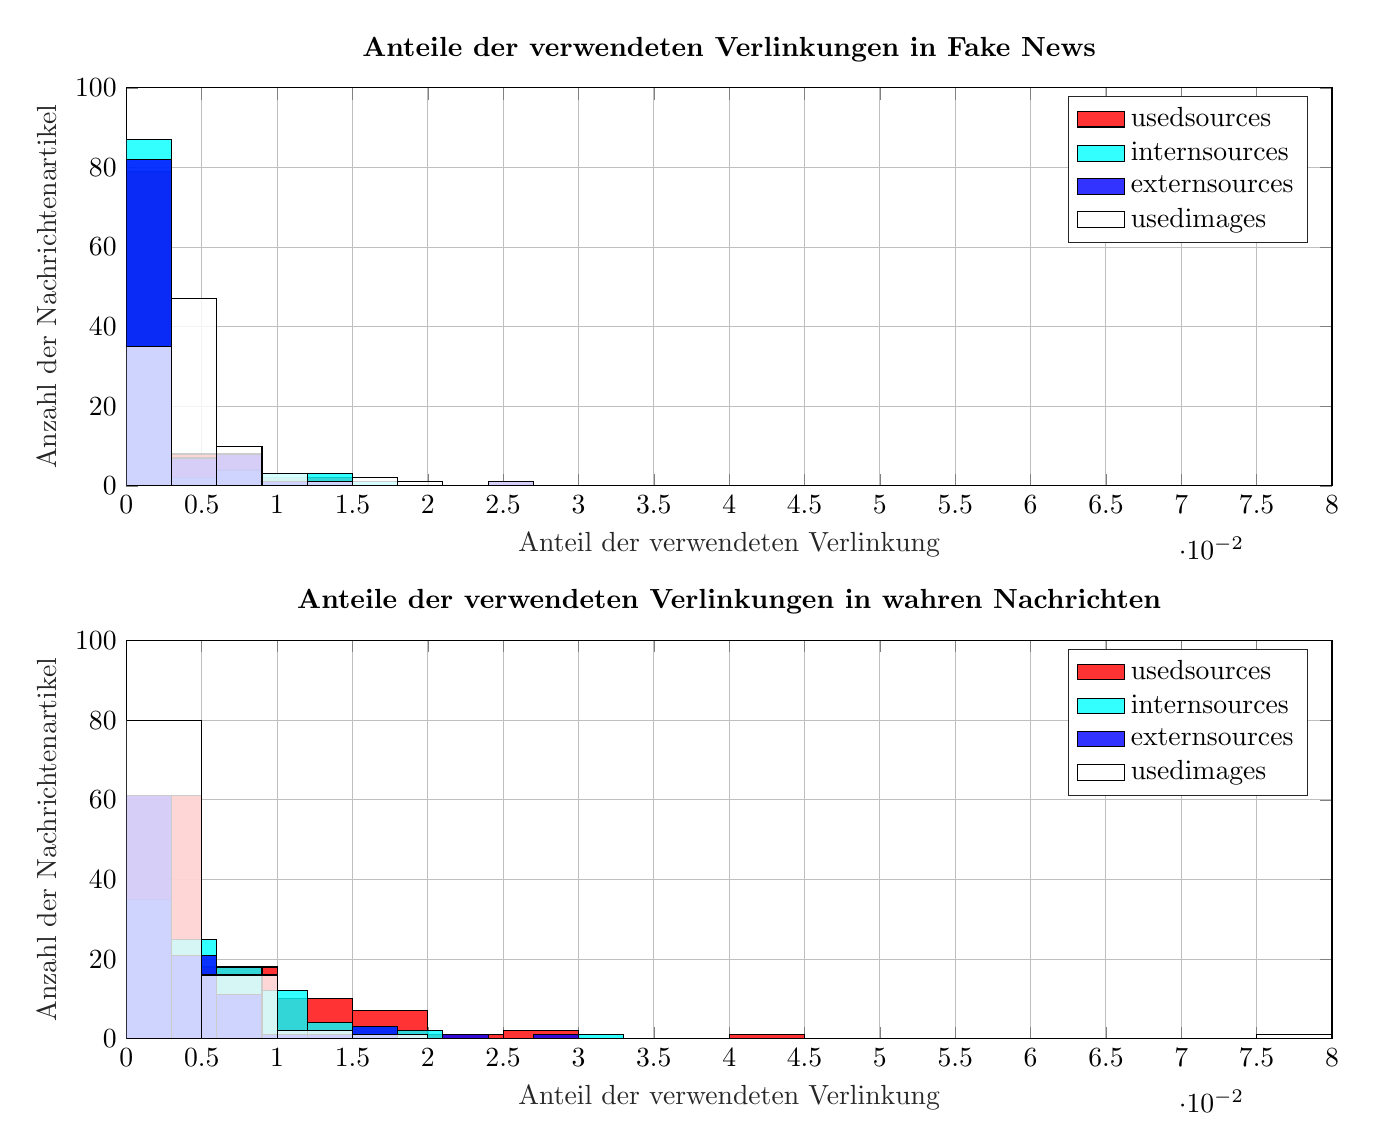
\begin{tikzpicture}

\begin{axis}[%
width=6.028in,
height=1.99in,
at={(1.011in,3.406in)},
scale only axis,
xmin=0,
xmax=0.08,
xlabel style={font=\color{white!15!black}},
xlabel={Anteil der verwendeten Verlinkung},
ymin=0,
ymax=100,
ylabel style={font=\color{white!15!black}},
ylabel={Anzahl der Nachrichtenartikel},
axis background/.style={fill=white},
title style={font=\bfseries},
title={Anteile der verwendeten Verlinkungen in Fake News},
xmajorgrids,
ymajorgrids,
legend style={legend cell align=left, align=left, draw=white!15!black}
]
\addplot[ybar interval, fill=red, fill opacity=0.8, draw=black, area legend] table[row sep=crcr] {%
x	y\\
0	79\\
0.003	8\\
0.006	8\\
0.009	2\\
0.012	2\\
0.015	0\\
0.018	0\\
0.021	0\\
0.024	1\\
0.027	1\\
};
\addlegendentry{usedsources}

\addplot[ybar interval, fill=mycolor1, fill opacity=0.8, draw=black, area legend] table[row sep=crcr] {%
x	y\\
0	87\\
0.003	2\\
0.006	4\\
0.009	3\\
0.012	3\\
0.015	1\\
0.018	1\\
};
\addlegendentry{internsources}

\addplot[ybar interval, fill=blue, fill opacity=0.8, draw=black, area legend] table[row sep=crcr] {%
x	y\\
0	82\\
0.003	7\\
0.006	8\\
0.009	1\\
0.012	1\\
0.015	0\\
0.018	0\\
0.021	0\\
0.024	1\\
0.027	1\\
};
\addlegendentry{externsources}

\addplot[ybar interval, fill=white, fill opacity=0.8, draw=black, area legend] table[row sep=crcr] {%
x	y\\
0	35\\
0.003	47\\
0.006	10\\
0.009	3\\
0.012	1\\
0.015	2\\
0.018	1\\
0.021	0\\
0.024	1\\
0.027	1\\
};
\addlegendentry{usedimages}

\end{axis}

\begin{axis}[%
width=6.028in,
height=1.99in,
at={(1.011in,0.642in)},
scale only axis,
xmin=0,
xmax=0.08,
xlabel style={font=\color{white!15!black}},
xlabel={Anteil der verwendeten Verlinkung},
ymin=0,
ymax=100,
ylabel style={font=\color{white!15!black}},
ylabel={Anzahl der Nachrichtenartikel},
axis background/.style={fill=white},
title style={font=\bfseries},
title={Anteile der verwendeten Verlinkungen in wahren Nachrichten},
xmajorgrids,
ymajorgrids,
legend style={legend cell align=left, align=left, draw=white!15!black}
]
\addplot[ybar interval, fill=red, fill opacity=0.8, draw=black, area legend] table[row sep=crcr] {%
x	y\\
0	61\\
0.005	18\\
0.01	10\\
0.015	7\\
0.02	1\\
0.025	2\\
0.03	0\\
0.035	0\\
0.04	1\\
0.045	1\\
};
\addlegendentry{usedsources}

\addplot[ybar interval, fill=mycolor1, fill opacity=0.8, draw=black, area legend] table[row sep=crcr] {%
x	y\\
0	35\\
0.003	25\\
0.006	18\\
0.009	12\\
0.012	4\\
0.015	3\\
0.018	2\\
0.021	0\\
0.024	0\\
0.027	0\\
0.03	1\\
0.033	1\\
};
\addlegendentry{internsources}

\addplot[ybar interval, fill=blue, fill opacity=0.8, draw=black, area legend] table[row sep=crcr] {%
x	y\\
0	61\\
0.003	21\\
0.006	11\\
0.009	1\\
0.012	1\\
0.015	3\\
0.018	0\\
0.021	1\\
0.024	0\\
0.027	1\\
0.03	1\\
};
\addlegendentry{externsources}

\addplot[ybar interval, fill=white, fill opacity=0.8, draw=black, area legend] table[row sep=crcr] {%
x	y\\
0	80\\
0.005	16\\
0.01	2\\
0.015	1\\
0.02	0\\
0.025	0\\
0.03	0\\
0.035	0\\
0.04	0\\
0.045	0\\
0.05	0\\
0.055	0\\
0.06	0\\
0.065	0\\
0.07	0\\
0.075	1\\
0.08	1\\
};
\addlegendentry{usedimages}

\end{axis}
\end{tikzpicture}%